\documentclass{acm_proc_article-sp}
\usepackage{caption,subcaption}

\begin{document}

\title{Using Information Theoretic Criteria to Discover Useful Options}


\numberofauthors{2} %  in this sample file, there are a *total*
% of EIGHT authors. SIX appear on the 'first-page' (for formatting
% reasons) and the remaining two appear in the \additionalauthors section.
%
\author{
% You can go ahead and credit any number of authors here,
% e.g. one 'row of three' or two rows (consisting of one row of three
% and a second row of one, two or three).
%
% The command \alignauthor (no curly braces needed) should
% precede each author name, affiliation/snail-mail address and
% e-mail address. Additionally, tag each line of
% affiliation/address with \affaddr, and tag the
% e-mail address with \email.
%
% 1st. author
\alignauthor
Viktoria Kovecses\\
       \affaddr{McGill University}\\
       \email{viktoria.kovecses@mail.mcgill.ca}
% 2nd. author
\alignauthor
Doina Precup\\
       \affaddr{McGill University}\\
       \email{dprecup@cs.mcgill.ca}
}

\maketitle
\begin{abstract}

	Reinforcement learning allows autonomous agents to compute optimal ways of behaving by interacting with an environment. Temporally extended actions, or options, allow algorithms to achieve faster convergence to an optimal policy. While options can be defined manually for some MDPs, this is difficult in general because it may be unclear what options are good without prior knowledge of the environment. Therefore, it is beneficial to find good options automatically. We propose a novel approach which creates random options and then sifts through them using an information theoretic policy search algorithm. The algorithm combines a measure of predictive information and rewards to guide the agent. Our approach shows promising empirical results on small navigation problems and is computationally efficient. 
	
\end{abstract}

% A category with the (minimum) three required fields
\category{H.4}{Information Systems Applications}{Miscellaneous}
%A category including the fourth, optional field follows...
\category{D.2.8}{Software Engineering}{Metrics}[complexity measures, performance measures]

\terms{Theory}

\keywords{finding options, information theory, predictive information} % NOT required for Proceedings

\section{Introduction}
%Talk about the work in general. This section is to introduce what we will do and its significance so talk about why options in general are important, and then talk a bit about background and how we will be adding to the already existing research in this area. 

%Explain temporal abstraction a bit...
%what would be a good example for this? 
%From Solway: Simple actions fit together into coherent subasks, which themselves combine to accomplish higher-level goals. This kind of tiered or nested structure is readily apparent in our everyday activities: Turning on the stove forms part of boiling water, which in turn forms part of cooking pasta.
People often use different levels of planning to execute their everyday actions. For instance, the action of making an appointment may consist of many sub-actions, such as picking up the phone, dialling the number, and speaking to the receptionist. The abstraction of sub-actions into larger more compact actions is therefore useful in everyday life. However, it may also be useful in the context of reinforcement learning.

Temporal abstraction of actions has proved to be a useful tool allowing for faster convergence of algorithms to an optimal policy in Markov Decision Processes (MDPs). These temporally abstracted actions are often referred to as options, and they in general consist of a set of states, a policy, and termination conditions. 

Although options may be a very powerful tool once created, they are not always easy to instantiate manually. In some environments the state space may be simply too large, while in others it may not be evident what a good option would consist of. Therefore, it would be beneficial to be able to generate options programmatically for any given environment.

Previous work on finding useful options has shown that for at least some environments it is beneficial to define the option in such a way that the goal state of the subpolicy is a bottleneck (e.g. a hallway between rooms) \cite{solwayoptimal}. However, this method fails if for instance the bottleneck happens to have a very negative reward. Another method for finding options is to look at solutions to several tasks in the same environment, and observe where the optimal actions overlap \cite{pickett2002policyblocks}. The states where the actions remain constant across tasks can then be used to make options.

In our project, instead of trying to understand what makes a good option by first observing interesting parts of the environment and then creating options, we instead create several random options and observe how an information theoretic driven policy search algorithm \cite{still} chooses between options and actions. Essentially, we would like to examine whether using predictive information (i.e. $I[(A_t,X_t); X_{t+1}]$) as well as the return in the environment could be useful in finding decent options for any given MDP.

\section{Background} %title?

Very general overview of what we did and maybe a bit about the results though I'm not sure that is necessary. A bit like an outline of the paper (i.e. we will first discuss this and then show that).

\subsection{Reinforcement Learning}

%Explain reinforcement learning in general. Basically the first paragraph of the extended abstract in a bit more detail.

The reinforcement learning framework involves an agent learning about an environment by interacting with it across discrete time steps. To accomplish this the agent moves around by taking different actions, and accumulating rewards as it goes.
	 The environment is often modelled as a Markov Decision Process (MDP) \cite{Puterman}, which consists of a set of states $\mathcal{S}$, a set of actions $\mathcal{A}$, a transition probability matrix $\mathcal{P}$, and a reward function $\mathcal{R}$. Each state represents a portion of the environment, while the actions can be applied to take the agent from one state to another. 
	 The transition probability matrix contains the probability that the agent ends up at state $s_{t+1}$ if it takes action $a_t$ in state $s_t$ at time t. Finally, the reward function indicates the reward $r_{t+1}$ that the agent obtains by taking action $a_t$ in state $s_t$. In addition, the agent may act according to a policy $\pi$, which is a mapping of actions to states that indicates the action to take at each state. The goal of the agent now becomes to maximize the accumulated reward by finding an optimal policy in the environment.  
	 
\subsection{Options}

%Explain options here.

In many situations it may be beneficial to use temporal abstraction to allow the agent to plan using different levels in the environment. For example, if we wish the agent to walk straight until it reaches an obstacle in a continuous environment, we may not want to tell it what to do at each state but simply tell it to move in the same direction for a certain period of time. This would be an example of a temporally abstracted action.

By defining a fixed subpolicy for a group of states in an MDP before the agent begins exploration, one can achieve a faster convergence to an optimal policy. More formally, we may refer to these as options, which are made up of three parts: an initiation set, a policy, and termination conditions \cite{sutton1999between}. The initiation set, a subset of the state space, includes all the states where the option can be executed, the policy represents how the agent should act in each of these states, and the termination condition is the probability that the option will terminate at any given state \cite{sutton1999between}.

\subsection{Information Theory Aspect}

Maybe give a different title to this subsection. Talk about the information theory aspect and its importance in the research. Link it to options.

\subsubsection{Predictive Information}

%Define mutual information, and explain the concept of predictive information.

In information theory mutual information is often defined as the information that a random variable X carries about a random variable Y, and vice versa. In other words, it tells us how well knowing one of the random variables can help us predict the other, and is calculated as follows:

\[I(X; Y) = \sum_{x \in X}\sum_{y \in Y}p(x,y)log(\frac{p(x,y)}{p(x)p(y)})\]

The predictive information is then defined to be the information that the current state and action carry about the state the agent will end up in next (i.e. $I[(A_t,X_t); X_{t+1}]$). It can also be thought of as a measure of the ability of the agent to predict where it will move if it takes an action at its current state. 

\subsubsection{Kullback-Leibler Divergence}

%Not sure if this should have its own subsection but maybe explain how we will increase predictive information in the algorithm. Basically a general explanation of how the algorithm will work. Maybe have the entire algorithm as a figure.

The Kullback-Leibler divergence between two probability distributions is defined as follows: 
\[D_{KL}(p || q) = \sum_{x \in X} p(x)log(\frac{p(x)}{q(x)})\]

It essentially measures the difference between two probability distributions $p$ and $q$. For instance, if the two probability distributions are identical, the divergence would be 0, and if they are very different then the divergence may go to infinity.

In order to maximize the predictive information, as the information theoretic aspect of the algorithm aims to do, we do not directly calculate the predictive information using the mutual information formula, but instead use the Kullback-Leibler divergence between the transition probabilities (i.e. the true model) and the empirically calculated steady state distribution: $D_{KL}(p(X_{t+1}|a, x_t) || p^\pi(X_{t+1}))$. If we consider the steady state distribution $p^\pi(X_{t+1})$ to be an approximation of the transition probability distribution, then we can use the divergence as a measure of the predictive information. For example, if the steady state distribution is very different from the transition probability distribution, then what the agent observes about the environment is not yet close to what the agent expects to see. Therefore, more exploration is required to reduce the divergence and hopefully bring the steady state distribution closer to the transition probability distribution if possible. 

\subsubsection{Algorithm} %title?

%Explain the algorithm, maybe include a figure.

The algorithm used in our research was taken from previous work completed by Doina Precup and Suzanne Still \cite{still}. It is a policy search algorithm which takes into account both the predictive information in the environment (i.e. $I[(A_t,X_t); X_{t+1}]$), as well as the return in order to compute an optimal deterministic policy which may be tuned to encourage a certain amount of exploration in the environment. The policy is computed at each time step using the following equation: $$q_{opt}(A_t = a| X_t = x) = \frac{p_t(a)e^{\frac{1}{\lambda}*(D(x,a) + \alpha*Q(x,a))}}{Z(x)}$$ where $D(x,a)$ represents the Kullback-Leibler divergence between the true model and an estimated steady state distribution, or how well the estimated model predicts the true model; and $Q(x,a)$ represents the action values as in usual reinforcement learning.

\subsection{Experiments}

Explain the different experiments that were done as well as the environments that were used.

\subsubsection{Grid Environments}

%add a figure of the grid environment

For the experiments, different variations of a simple 10 x 10 grid world were created. They all contained at a start and a goal state, and the dynamics of the environment remained constant across variations. The agent would always start from the start state and try to move towards the goal which had a reward of +1. The reward everywhere else was 0. The action space contained four primitive actions which the agent could take, namely $up, down, left$, and $right$; and these actions simply moved the agent towards the corresponding adjacent square. For any primitive action taken, there was a 0.7 probability that the action would succeed, and in the event of failure a different action would be chosen randomly. 

%A few of the experiments were also conducted on a 10 x 10 grid world identical to the one previously described, except for this grid world did not contain any obstacles, and therefore had many possible paths from the start to the goal.

%For the majority of experiments, a 10 x 10 grid environment was used (see figure). It contained a start and goal state, as well as obstacles arranged to make two distinct paths between the start and the goal. Though both paths were of equal length, one of the paths (top) was straightforward and made it easy to reach the goal, whereas the other path was winding and less obvious. The agent would always start from the start state and try to move towards the goal which had a reward of +1. The reward everywhere else was 0. The action space contained four primitive actions which the agent could take, namely $up, down, left$, and $right$; and these actions simply moved the agent towards the corresponding adjacent square. For any primitive action taken, there was a 0.7 probability that the action would succeed, and in the event of failure a different action would be chosen randomly. 

\subsubsection{Interesting area}

In order to test whether the information theoretic criteria had any influence in the agent's exploration, an area of interest was added to some of the grid environments (see figure). This area consisted of a set of states in which either the reward or the probability of an action succeeding would vary based on a Gaussian or Uniform probability distribution, respectively. In the case that the reward was varied, the average reward remained 0, and therefore going through this area to reach the goal ultimately made no difference in reward for the agent compared to other paths.

%\subsubsection{Empty Grid World}

\subsection{Results}

Give the results to the experiments and say whether they are good/bad and what they teach us. Include a few figures here and hopefully there will be graphs.

%Giant option
In Figure 1, the algorithm is used on a grid world with a large random option, composed of every state except the subgoal where the option terminates. The policy found only includes the option if it moves the agent closer to the goal from most states, and leads to improved performance when it is used. This shows the ability of this technique to sift through options and potentially make it easier to find good options without making any assumptions about the environment.

%Giant option
\begin{figure*}[!htbp]
  \begin{subfigure}[h]{.5\textwidth}
  	\centering
    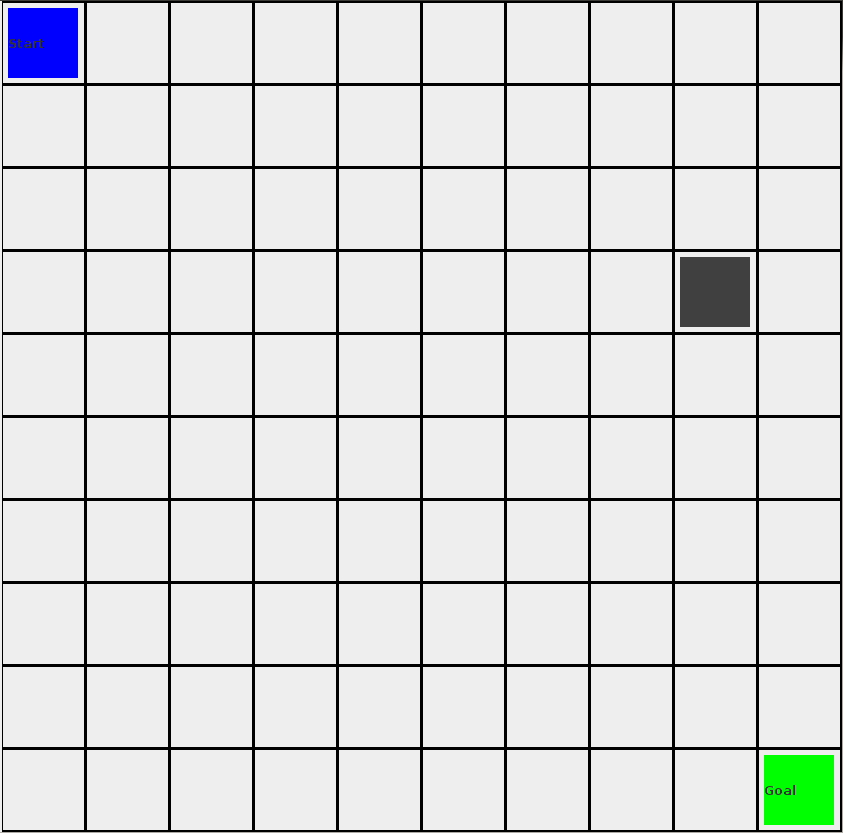
\includegraphics[width=2.5in]{GiantOp1.png}
    \caption{Option which leads most states away from the goal}
  \end{subfigure}\hfill
  \begin{subfigure}[h]{.5\textwidth}
  \centering
    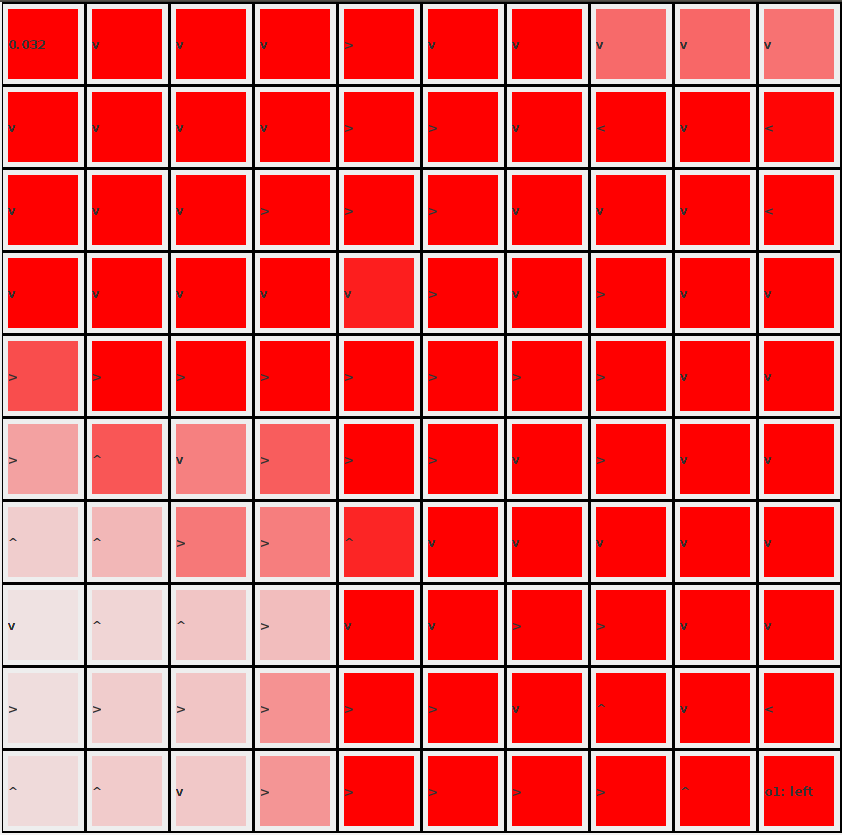
\includegraphics[width=2.5in]{GiantOption1Pol.png}
    \caption{Option (from (a)) is not selected in any of the states}
  \end{subfigure}
  \hfill
  \begin{subfigure}[h]{.5\textwidth}
  \centering
    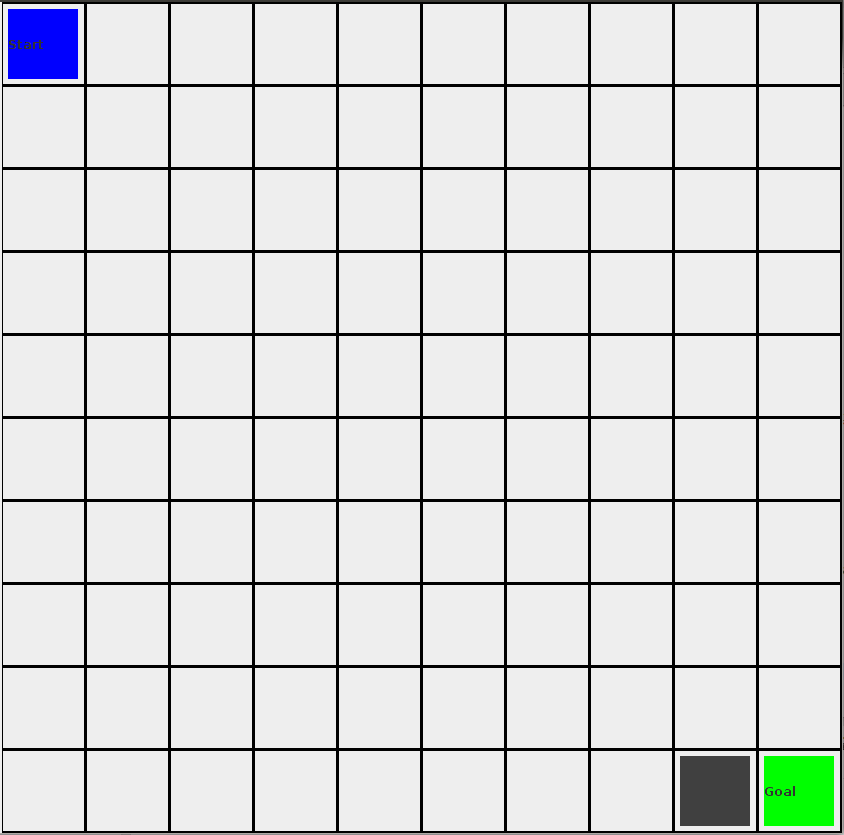
\includegraphics[width=2.5in]{GiantOp2.png}
    \caption{Option which leads most states towards the goal}
  \end{subfigure}
  \hfill
  \begin{subfigure}[h]{.5\textwidth}
  \centering
    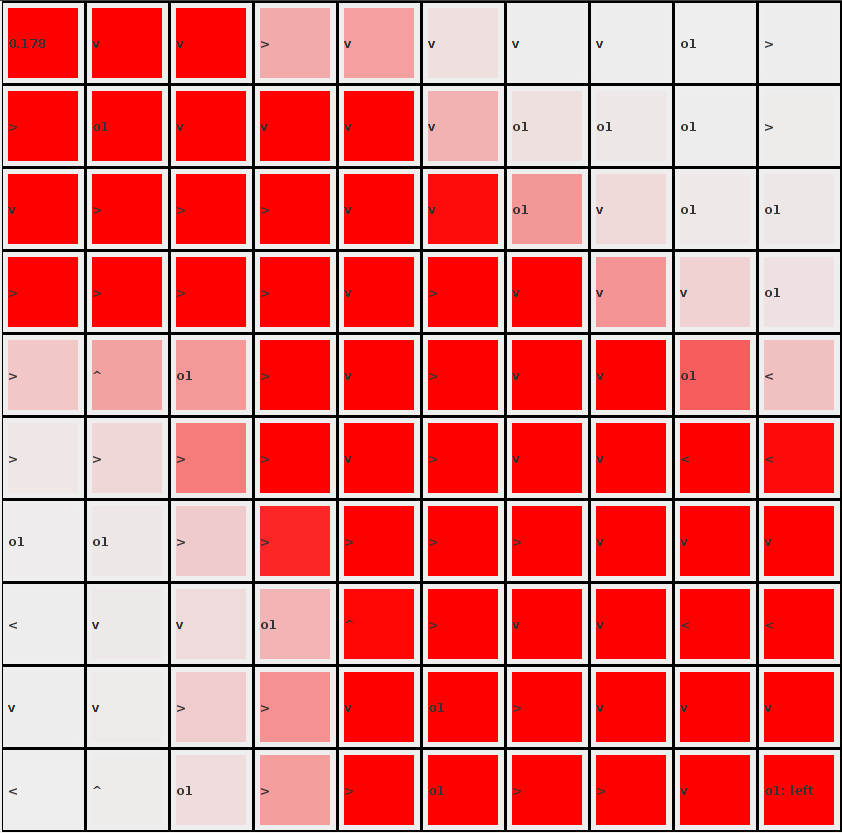
\includegraphics[width=2.5in]{GiantOp2Pol.png}
    \caption{Option (from (c)) is selected in several states}
  \end{subfigure}
  \caption{Results of testing the algorithm on an obstacle-free environment with one large random option. In (a) and (c) the blue tile represents the starting state, the green tile represents the goal, and the black tile is the subgoal for the option. In (b) and (d), a darker red represents states that were visited more frequently.}
  \vspace{20pt}
\end{figure*}

%Grid world with interesting area
	%show how path with interesting area is preferred
	%maybe redo this experiment

%Experiment with many runs averaged
In another experiment, a similar grid world was used, with this one now containing a large square obstacle in the center. This left for two paths of equal length to the goal, each of which contained a hand-crafted option leading the agent down the path and towards the goal (see Figure 2). The sole difference between the two paths was that the left-most path contained a subset of states, called the "interesting area", in which the probability of an action succeeding varied from 0 to 1 uniformly randomly.
	 The interest of the experiment was to see how the options would be selected along either path, and if the area where actions succeed randomly would affect the policy. The results showed that along both paths the options were initially preferred, and quickly increased the overall return. 
	 However, in the states examined the algorithm traded the option for the optimal primitive action, which also happened to be the same action the option was executing in that state. The policy thus switched to consist mainly of primitive actions, though there was no significant change in the return. This shows that the useful options are incorporated into the policy, and only get traded for the optimal primitive action, which is expected as this leads to an improved and simpler policy in most cases.
	  It can also be noted that the policy selected the optimal primitive action very early on, and this action remained dominant until the completion of the algorithm. The reason for this is most likely that the Q value for the chosen action quickly became higher than the Q values for all other actions, even surpassing the options, thus giving this action a significant advantage.
	  The same results were found when observing states in the interesting area; however, in these states there were slightly greater fluctuations in the policy, most likely due to the high uncertainty of actions succeeding.
	  
%averaged many runs
\begin{figure*}[!htbp]
  \begin{subfigure}[h]{.4\textwidth}
  	\centering
    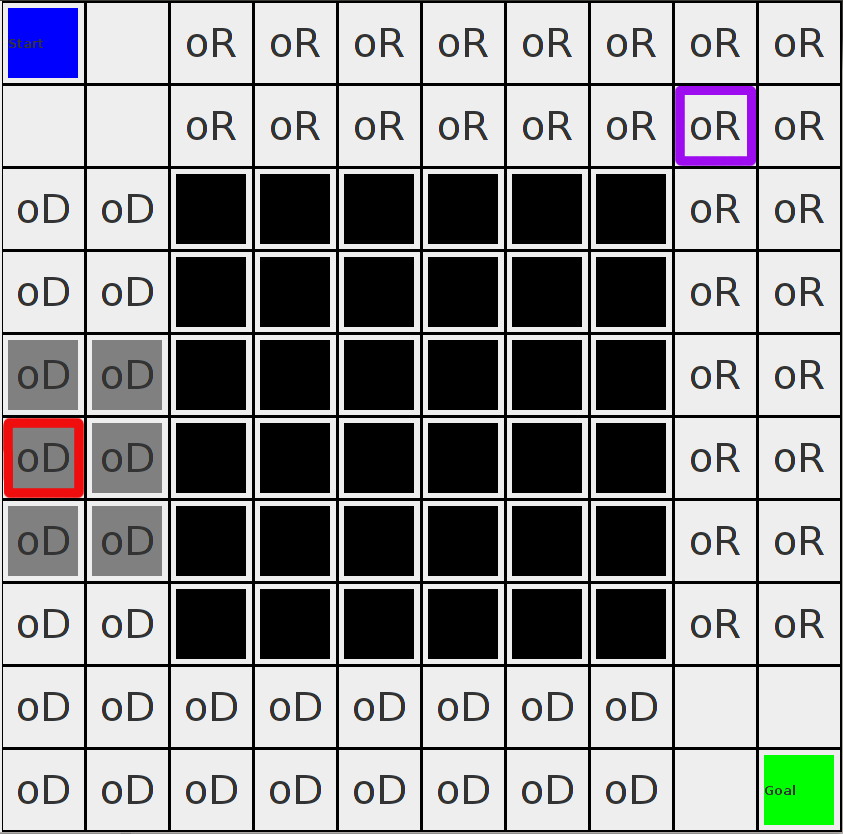
\includegraphics[width=2in]{ops.png}
    \caption{Environment with square obstacle, and two large options leading towards the goal (oD and oR). Blue square: start, Green square: Goal, Grey squares: interesting area, Purple outline: State 18, Red outline: State 50}
  \end{subfigure}\hfill
  \begin{subfigure}[h]{.45\textwidth}
  \centering
    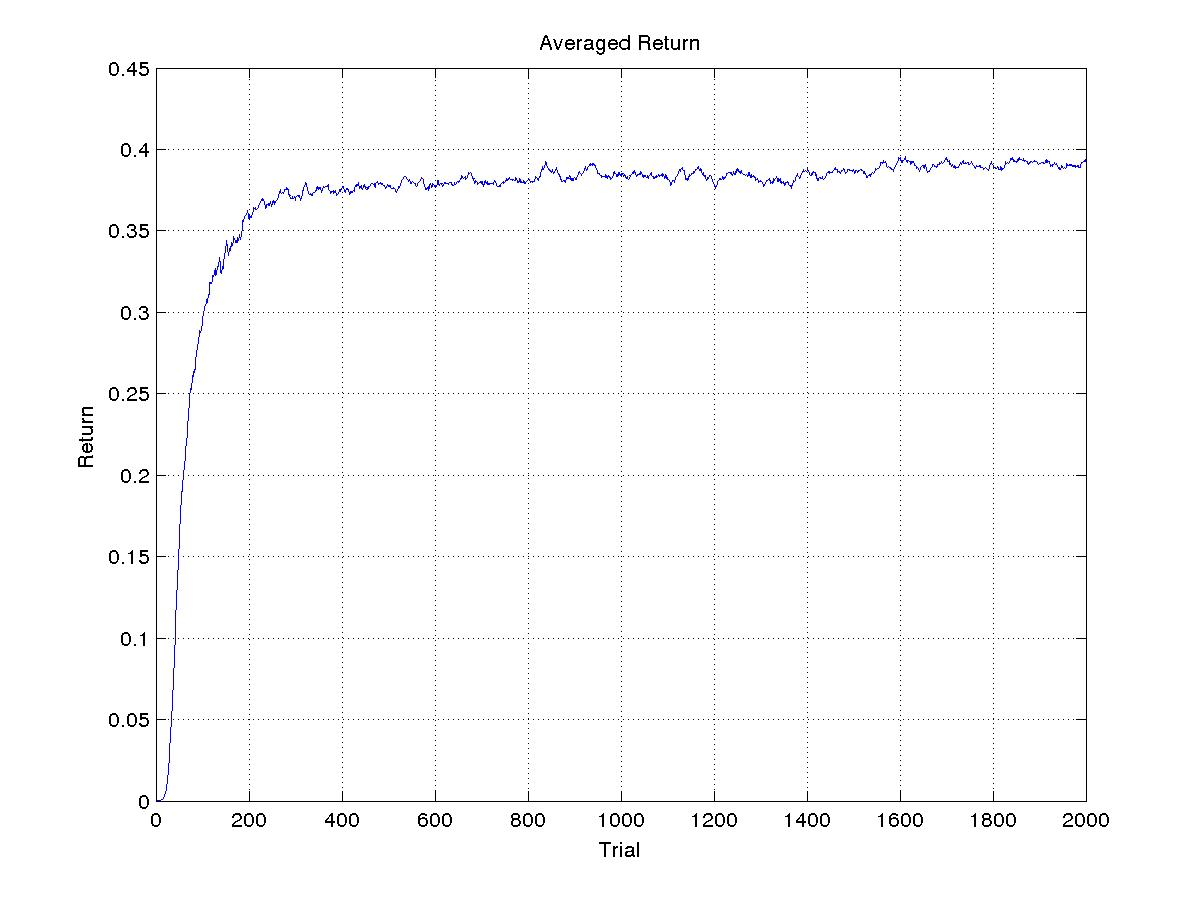
\includegraphics[width=3.5in]{return.jpeg}
    \caption{Average return accumulated over time}
  \end{subfigure}
  \hfill
  \begin{subfigure}[h]{.45\textwidth}
  \centering
    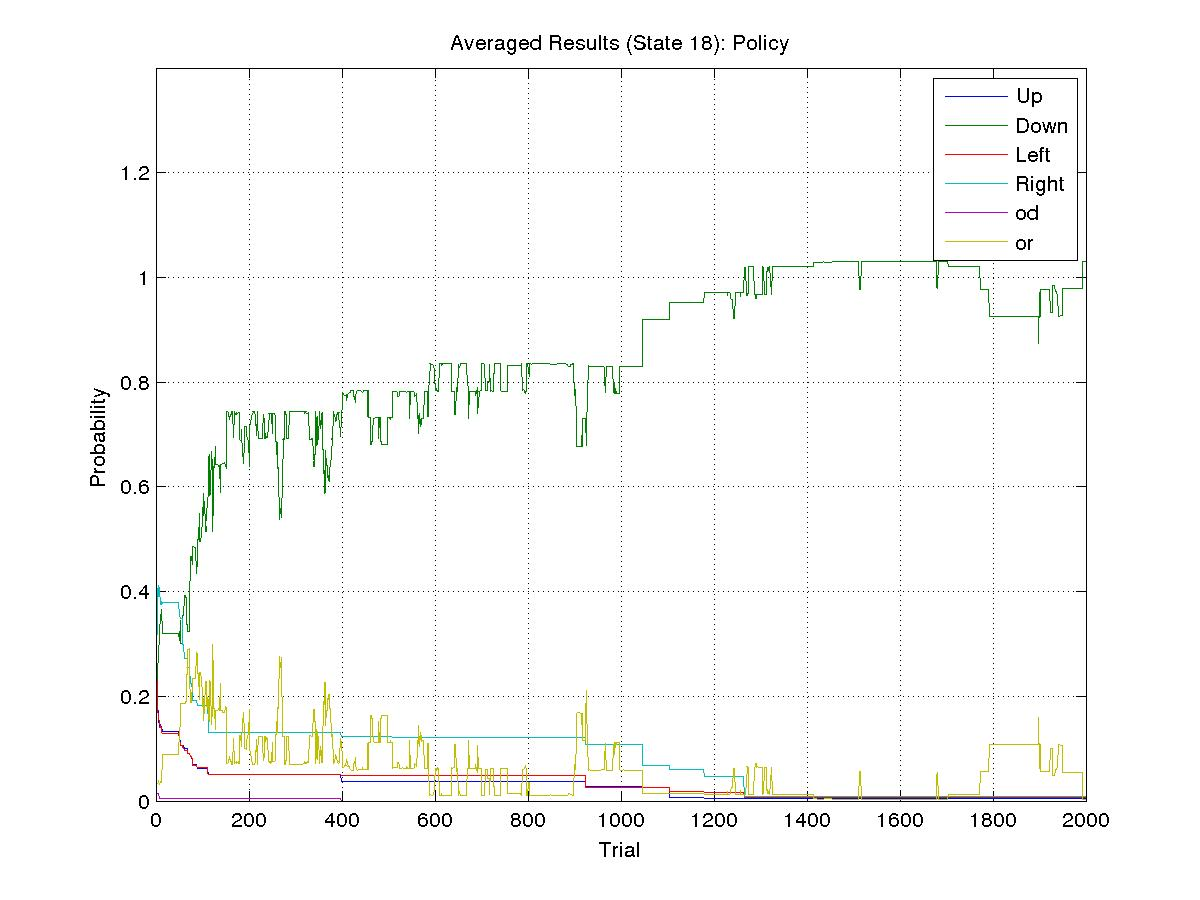
\includegraphics[width=3.5in]{pol18.jpeg}
    \caption{Policy over time at state 18. Green line: Probability of taking down action, Yellow line: Probability of taking option oR}
  \end{subfigure}
  \hfill
  \begin{subfigure}[h]{.45\textwidth}
  \centering
    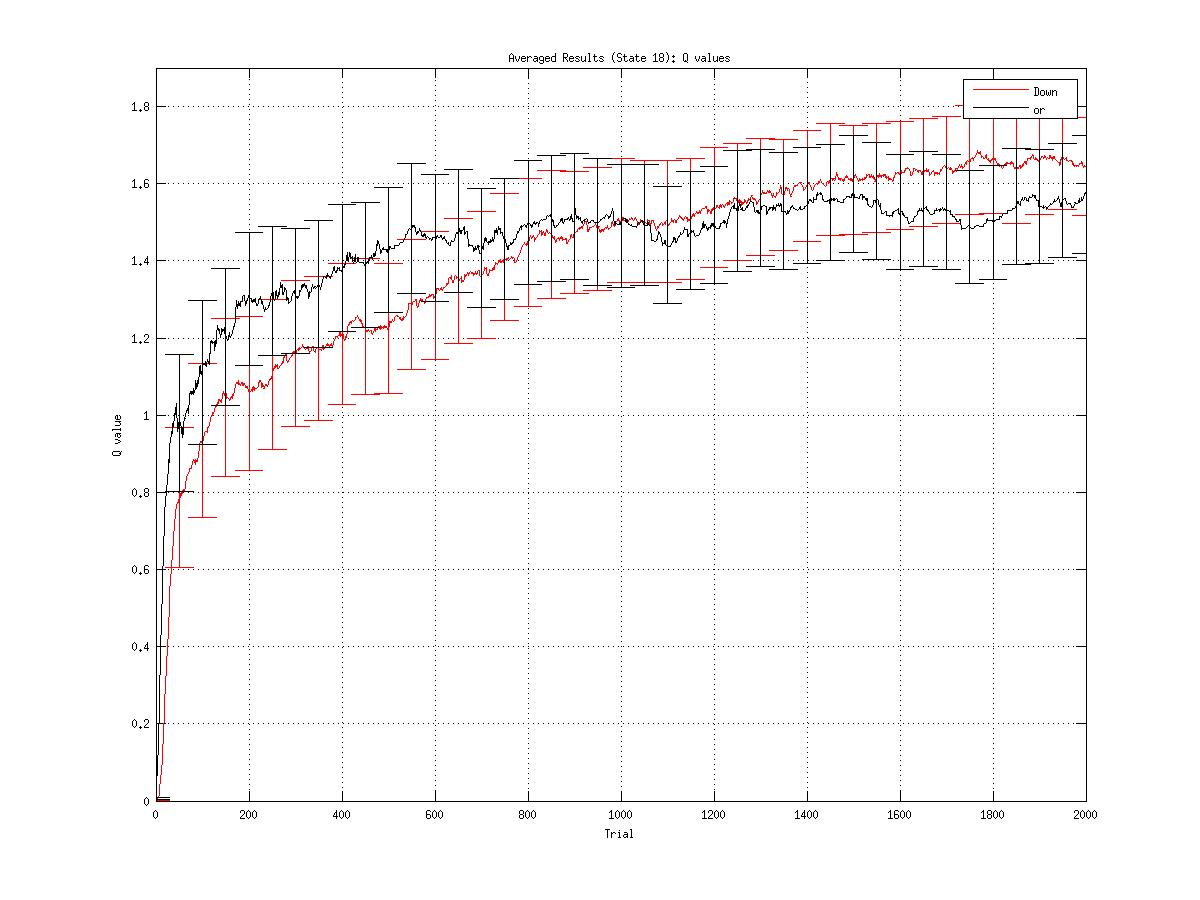
\includegraphics[width=3.5in]{Q18.jpeg}
    \caption{Q values over time at state 18. Green line: Q value for down action, Yellow line: Q value for option oR}
  \end{subfigure}
    \hfill
  \begin{subfigure}[h]{.45\textwidth}
  \centering
    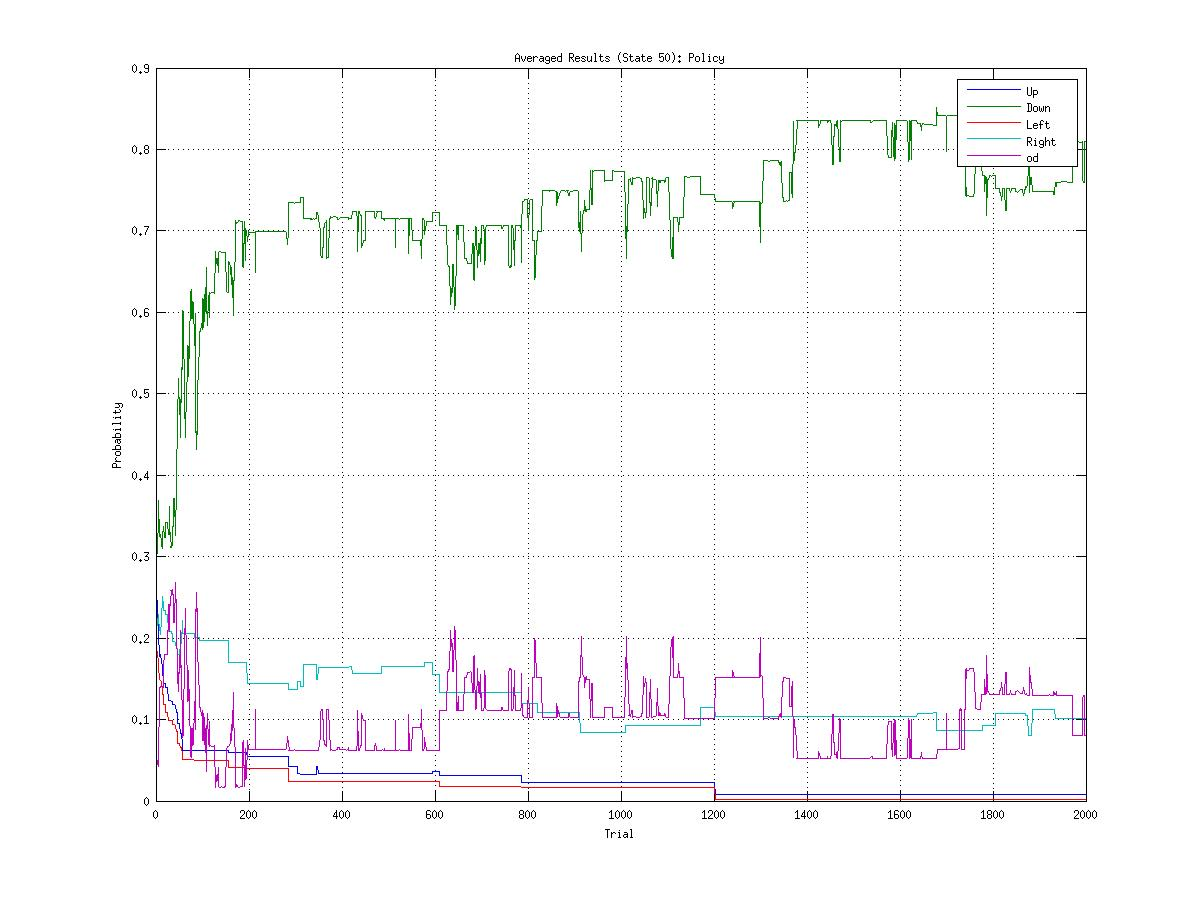
\includegraphics[width=3.5in]{pol50.jpeg}
    \caption{Policy over time at state 50. Green line: Probability of taking down action, Purple line: Probability of taking option oD}
  \end{subfigure}
    \hfill
  \begin{subfigure}[h]{.45\textwidth}
  \centering
    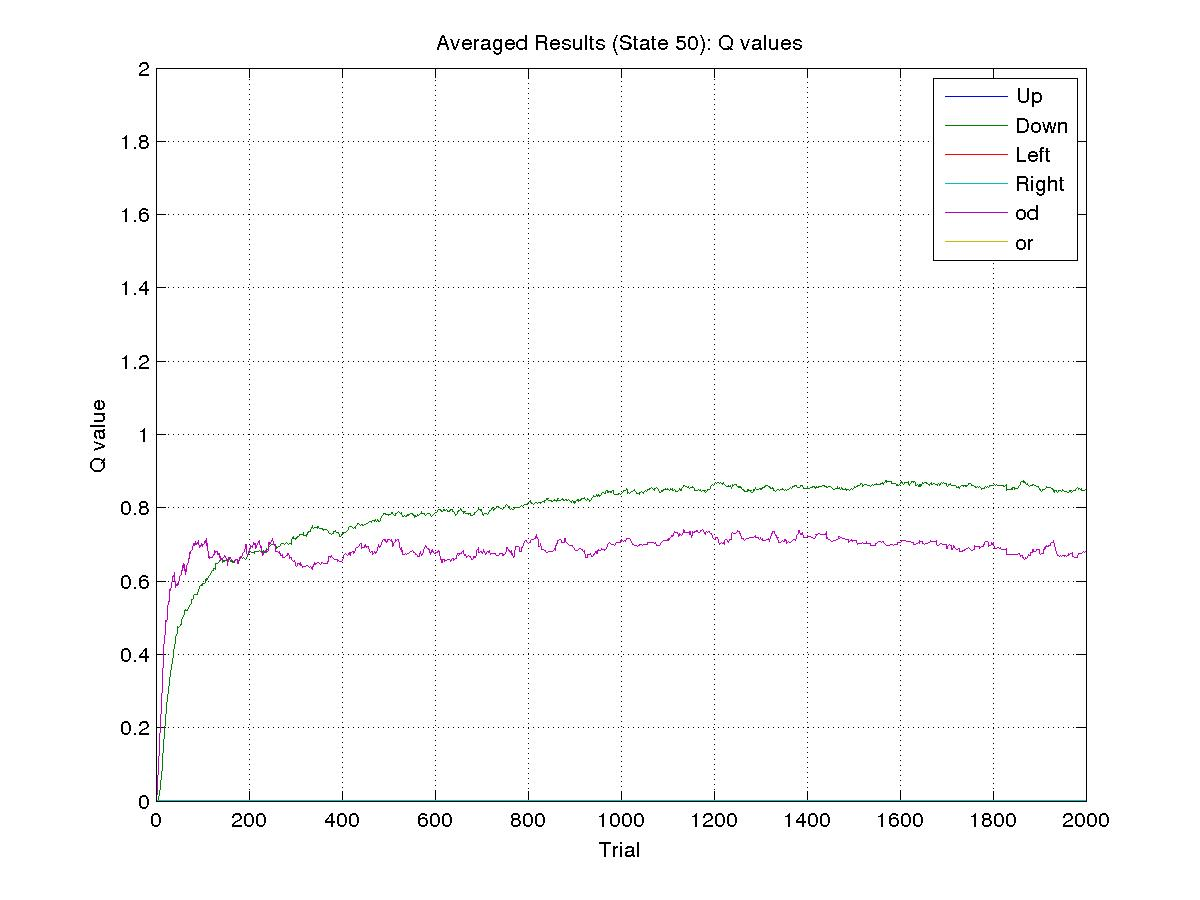
\includegraphics[width=3.5in]{Q50.jpeg}
    \caption{Q values over time at state 50. Green line: Q value for down action, Purple line: Q value for option oD}
  \end{subfigure}
  \caption{Results of running the algorithm on an environment with one large obstacle and two hand-crafted options. The results are averaged over 20 full runs of the algorithm.}
  \vspace{20pt}
\end{figure*}

\section{Conclusions}

Summarize results and there significance, talk about future work that could be done.

%future work
More work is still needed to see whether this method would work well in different settings, and to compare it to other option finding algorithms. Furthermore, using different aspects of information theory, such as entropy instead of predictive information may be interesting to explore as well.
%\end{document}  % This is where a 'short' article might terminate

%ACKNOWLEDGMENTS are optional
\section{Acknowledgments}
This section is optional; it is a location for you
to acknowledge grants, funding, editing assistance and
what have you.  In the present case, for example, the
authors would like to thank Gerald Murray of ACM for
his help in codifying this \textit{Author's Guide}
and the \textbf{.cls} and \textbf{.tex} files that it describes.

%
% The following two commands are all you need in the
% initial runs of your .tex file to
% produce the bibliography for the citations in your paper.
\bibliographystyle{abbrv}
\bibliography{references}  % sigproc.bib is the name of the Bibliography in this case
% You must have a proper ".bib" file
%  and remember to run:
% latex bibtex latex latex
% to resolve all references
%
% ACM needs 'a single self-contained file'!
%
%APPENDICES are optional
%\balancecolumns
\appendix
%Appendix A
\section{Headings in Appendices}
The rules about hierarchical headings discussed above for
the body of the article are different in the appendices.
In the \textbf{appendix} environment, the command
\textbf{section} is used to
indicate the start of each Appendix, with alphabetic order
designation (i.e. the first is A, the second B, etc.) and
a title (if you include one).  So, if you need
hierarchical structure
\textit{within} an Appendix, start with \textbf{subsection} as the
highest level. Here is an outline of the body of this
document in Appendix-appropriate form:
\subsection{Introduction}
\subsection{The Body of the Paper}
\subsubsection{Type Changes and  Special Characters}
\subsubsection{Math Equations}
\paragraph{Inline (In-text) Equations}
\paragraph{Display Equations}
\subsubsection{Citations}
\subsubsection{Tables}
\subsubsection{Figures}
\subsubsection{Theorem-like Constructs}
\subsubsection*{A Caveat for the \TeX\ Expert}
\subsection{Conclusions}
\subsection{Acknowledgments}
\subsection{Additional Authors}
This section is inserted by \LaTeX; you do not insert it.
You just add the names and information in the
\texttt{{\char'134}additionalauthors} command at the start
of the document.
\subsection{References}
Generated by bibtex from your ~.bib file.  Run latex,
then bibtex, then latex twice (to resolve references)
to create the ~.bbl file.  Insert that ~.bbl file into
the .tex source file and comment out
the command \texttt{{\char'134}thebibliography}.
% This next section command marks the start of
% Appendix B, and does not continue the present hierarchy
\section{More Help for the Hardy}
The acm\_proc\_article-sp document class file itself is chock-full of succinct
and helpful comments.  If you consider yourself a moderately
experienced to expert user of \LaTeX, you may find reading
it useful but please remember not to change it.
\balancecolumns
% That's all folks!
\end{document}
